\documentclass[10pt,portuguese]{article}
\usepackage[portuguese]{babel}

\usepackage{fourier}
\usepackage[bottom]{footmisc}

\usepackage[]{graphicx}
\usepackage[]{color}
\usepackage{xcolor}
\usepackage{alltt}
\usepackage{listings}
\usepackage[T1]{fontenc}
\usepackage[utf8]{inputenc}
\setlength{\parskip}{\smallskipamount}
\setlength{\parindent}{5ex}
\usepackage{indentfirst}
\usepackage{listings}
\usepackage{setspace}
\usepackage{hyperref}
\hypersetup{
    colorlinks=true,
    linkcolor=auburn,
    filecolor=magenta,      
    urlcolor=blue, urlsize=2em
}

% Set page margins
\usepackage[top=100pt,bottom=100pt,left=68pt,right=66pt]{geometry}

% Package used for placeholder text
\usepackage{lipsum}

% Prevents LaTeX from filling out a page to the bottom
\raggedbottom

\definecolor{javared}{rgb}{0.6,0,0} % for strings
\definecolor{javagreen}{rgb}{0.25,0.5,0.35} % comments
\definecolor{javapurple}{rgb}{0.5,0,0.35} % keywords
\definecolor{javadocblue}{rgb}{0.25,0.35,0.75} % javadoc

\lstset{language=Java,
basicstyle=\footnotesize\ttfamily,
keywordstyle=\color{javapurple}\bfseries,
stringstyle=\color{javared},
commentstyle=\color{javagreen},
morecomment=[s][\color{javadocblue}]{/**}{*/},
numbers=left,
numberstyle=\tiny\color{black},
stepnumber=2,
numbersep=10pt,
tabsize=4,
showspaces=false,
showstringspaces=false}


\usepackage{fancyhdr}
\fancyhf{} 
\fancyfoot[C]{\thepage}
\renewcommand{\headrulewidth}{0pt} 
\pagestyle{fancy}

\usepackage{titlesec}
\titleformat{\chapter}
   {\normalfont\LARGE\bfseries}{\thechapter.}{1em}{}
\titlespacing{\chapter}{0pt}{50pt}{2\baselineskip}

\usepackage{float}
\floatstyle{plaintop}
\restylefloat{table}

\usepackage[tableposition=top]{caption}


\definecolor{light-gray}{gray}{0.95}

\renewcommand{\contentsname}{Índice}

\begin{document}


\begin{titlepage}
	\clearpage\thispagestyle{empty}
	\centering
	\vspace{2cm}

	
	{\Large  Padrões e Desenho de Software \par}
	\vspace{0.5cm}
	{\small Professores: \\
	José Luis Oliveira\par
	Sérgio Matos\par}
	\vspace{4cm}
	{\Huge \textbf{Clean Code}} \\
	\vspace{1cm}
	\vspace{4cm}
	{\normalsize  Hugo Paiva, 93195
	   \par}
	 
	\vspace{2cm}

    
\includegraphics[scale=0.20]{logo_ua.png}
    
    \vspace{2cm}
    
	{\normalsize DETI \\ 
		Universidade de Aveiro \par}
		
	{\normalsize 05-06-2020 \par}
	\vspace{2cm}
		
	
	\pagebreak

\end{titlepage}
\tableofcontents{}
\clearpage

\section{Clean Code}
\subsection{Introdução}

\par \textit{Clean Code} é o conceito de um código fácil de entender e susceptível a mudanças que ganhou relevância em 2008, quando \textit{Robert Cecil Martin} o mostrou ao mundo através do seu livro \textit{Clean Code: A Handbook of Agile Software Craftsmanship}. Neste livro, \textit{Robert} apresenta ao detalhe as técnicas e princípio ideais para o desenvolvimento de software de fácil compreensão.

\par Um sistema é algo que nunca está terminado, que necessita sempre de ser atualizado, quer seja devido à implementação de novas funcionalidade, resolução de problemas ou, até, devido a se ter tornado obsoleto. Ao longo destes ciclos de desenvolvimento, de modo a reduzir os custos de manutenção, é imperial a utilização de código limpo. Uma fraca qualidade de código leva a uma grande carga cognitiva, sendo necessárias mais horas de trabalho para a resolução de problemas. O problema 
é tão relevante que o livro refere um rácio de 10 leituras de código até começar a escrita.

\par Um código limpo é, portanto, algo que leva tempo, atenção e dedicação mas que tem resultados visíveis.

\subsection{Princípios e Boas Práticas}

\par Estando profundamente associado à complexidade de um sistema, ou seja, quanto mais limpo está o código, menos complexidade o sistema tem, é natural que o estudo dos sintomas desta complexidade seja um fator relevante para a escrita de um código limpo. 

\par Com isto em mente, \textit{Robert} definiu alguns princípios e boas práticas para chegar ao conceito de \textit{Clean Code}, tendo em conta toda a sua experiência em programação desde os anos 70.  De entre os referidos no livro, destacaram-se os seguintes:

\begin{itemize}
    \item \textbf{Nomes Significativos}
    \item \textbf{Organização de Funções}
    \item \textbf{Organização das Classes e Estruturas de Dados}
    \item \textbf{Comentários Expressivos}
    \item \textbf{Formatação de Código}
    \item \textbf{Tratamento de Erros}
    \item \textbf{Testes Limpos}
\end{itemize}

\subsubsection{Nomes Significativos}

\par Tal como o próprio princípio diz, os nomes devem ser significativos e de grande importância para manter um código compreensível. Independentemente do tipo de nome (funções, variáveis, métodos, etc.), segundo este princípio, os nomes devem seguir dois pontos principais:

\begin{itemize}
    \item Ir diretos ao ponto, passando a sua ideia central
    \item Em caso de necessidade, utilizar nomes grandes sem preocupações, garantindo a sua compreensão
\end{itemize}

\clearpage

\par Dito isto, são de evitar exemplos deste tipo, onde é pouco perceptível qual o contexto do problema:

\begin{lstlisting}
int[] f; // frutas
\end{lstlisting}

\begin{lstlisting}
for (int l=0; l<50; l++) {
	if (f[l] == 1) {
	    f[l] = 2;
	}
}
\end{lstlisting}

\par Ao invés, deve-se utilizar abordagens do género:

\begin{lstlisting}
int fruitsAtHome;
\end{lstlisting}

\begin{lstlisting}
final int NUMBER_OF_FRUITS = 50;
for (int l=0; l<NUMBER_OF_FRUITS; l++) {
	if (fruitsAtHome[l] == ROTTEN) {
	    fruitsAtHome[l] = TRASH;
	}
}
\end{lstlisting}

\par Existem, no entanto, outros aspetos que devem ser tido em consideração. Evitar símbolos e emojis, utilizar nomes de facil pronunciação, utilizar verbos em métodos e nomes em classes e utilizar sempre as mesmas palavras para um determinado contexto (utilizar sempre get ao invés de fetch) são alguns destes aspetos.

\subsubsection{Organização de Funções}

\par Segundo o autor deste conceito, existem duas regras para a criação das funções:

\begin{itemize}
    \item As funções devem ser pequenas
    \item As funções devem ser ainda mais pequenas
\end{itemize}

\par O objetivo com este trocadilho de regras é manter as funções com o mínimo de funcionalidades possíveis, permitindo uma menor complexidade ao longo do programa e, utilizando os nomes significativos, o código deverá estar organizado de maneira a que qualquer pessoa consiga ver todos os percursos ao longo da execução do programa facilmente. Aliás, durante o livro, é referido que as funções apenas devem fazer uma coisa.

\par Deve-se, também, utilizar menos argumentos, evitando, novamente, o aumento de complexidade:
\begin{lstlisting}
Circle makeCircle(Point center, double radius);
\end{lstlisting}

\par A declaração desta função é, sem dúvida, mais clara que a seguinte:

\begin{lstlisting}
Circle makeCircle(double x, double y, double radius);
\end{lstlisting}

\par Basicamente, continua-se a tendência de manter a menor complexidade possível, evitando efeitos secundários para além do objetivo das funções, repetições de código (DRY -Don’t Repeat Yourself), \textit{output} de vários argumentos mas utilizando tratamento de erros.

\clearpage

\subsubsection{Organização das Classes e Estruturas de Dados}

\par As classes devem manter-se pequenas e respeitar ao máximo princípios como o da \textit{Single Responsibility Principle} e \textit{Open-Closed Principle}, mantendo apenas uma responsabilidade e permitindo extensões mas não modificações, novamente, devido à complexidade. 

\par Como consequência, todas as variáveis devem manter-se privadas ou, no máximo, \textit{protected}, de modo a permitir testes. A abstração dos dados passa a ser uma prioridade com a criação de interfaces mais concisas, passando, por exemplo, de:

\begin{lstlisting}
public interface Phone {
    double getBatteryCapacityInMah();
    double getMahOfEnergyRemaing();
}
\end{lstlisting}

\par Para:

\begin{lstlisting}
public interface Phone {
    double getPercentBatteryRemaining();
}
\end{lstlisting}

\par Toda a comunicação entre classes deve também ser reduzida, comunicando apenas com as que se relacionam de alguma forma como por exemplo, com objetos criados em seus métodos, com outros objetos passados como argumentos, etc.

\subsubsection{Comentários Expressivos}

\par Apesar dos comentários serem uma parte importante da legibilidade do código, é também relevante verificar se estes se justificam:


\begin{lstlisting}
// Verificar se o carro ja deixou de pagar IUC em Portugal
if (car.age>25 || (car.eletric == true))...
\end{lstlisting}

\par Neste caso, os comentários não são necessário. A abordagem mais correta seria algo deste género:

\begin{lstlisting}
if (!car.paysIuc())...
\end{lstlisting}

\Par A partir deste exemplo, é possível chegar à conclusão que um \textit{Clean Code} não precisa realmente de comentário, o código deve ser auto explicativo. Ainda assim, caso seja necessário a utilização de comentários, estes devem ser claros, informativos e dar ênfase aos pontos importantes e nunca deixar código comentado em ambientes de produção.

\subsubsection{Formatação de Código}

\par Sem formatação de código, este passaria a ser praticamente impossível de ler pelos desenvolvedores. Deve-se ter em atenção a formatação na vertical como na horizontal no entanto, é necessário identificar os casos onde esta é necessário. Comentários desnecessários e ordenação de funções começando pelas mais simples, são práticas incorretas na formatação vertical. No entanto, exceder 120 caracteres por linha é muito grave no que consta à formatação horizontal.

\begin{lstlisting}
public class Student{  
 private    int         number;  
 private    String      name; 
 
 public void    insertData(int   n, 
                                    String    na){  
  number = n;  
  name =    na;  
 }  
\end{lstlisting}

\Par Num caso destes, não faz sentido aplicar o alinhamento horizontal pois este dificulta a leitura dos tipos de dados bem como de outras informações relevantes.

\begin{lstlisting}
public class Student {
    private int number;
    private String name;

    public void insertData(int r, String na) {
        number = n;
        name = na;
    }
\end{lstlisting}

\Par Por outro lado, a formatação é muito vantajosa para para perceber em que contexto certas funções e variáveis estão, devido à profundidade no código, com recurso a espaços antes de si:

\begin{lstlisting}
public class Dog {
   public Dog(String name) {
      System.out.println("Passed Name is :" + name );
   }

   public static void main(String []args) {
      Dog myDog = new Dog( "Lazy" );
   }
}
\end{lstlisting}

\subsubsection{Tratamento de Erros}

\Par Tendo em conta que os erros no desenvolvimento de software são recorrentes, é dever dos programadores preparar os seus programas para lidar com eles mas, de forma clara, de modo a manter a limpeza do código.

\Par É aconselhada a utilização de exceções ao invés de \textit{returns}, principalmente devido à sua lógica (\textit{bug}) não ser escondida. Caso este seja utilizado, nunca se deve retornar \textit{null} pois teremos que lidar com ele, o que gera ainda mais problemas. 

\par Um código limpo tem, portanto, de apresentar robustez logo, deve ser garantida a consistência do programa mesmo quando os erros acontecem.

\subsubsection{Testes Limpos}

\Par Um código só é considerado limpo após passar uma séries de testes, também estes limpos.

\Par As principais regras que estes testes têm de seguir são de acordo com o acrónimo F.I.R.S.T:

\begin{itemize}
    \item \textbf{Fast} - Devem ser rápidos, permitindo a sua execução múltiplas vezes vezes
    \item \textbf{Independent} - Devem ser independentes, evitando erros em cascata
    \item \textbf{Repeatable} - Devem permitir a repetição do teste em qualquer ambiente (num portátil, sem internet...)
    \item \textbf{Self-Validating} - Devem retornar um \textit{boolean} para permitir saber eficazmente o resultado do teste
    \item \textbf{Timely} - Devem ser escritos antes do código, facilitando a sua execução no código e, também, pontuais
\end{itemize}

\clearpage

\subsection{Clean Code aplicado no Mundo}

\Par Como já foi referido, um código limpo é algo que leva tempo, atenção e dedicação, algo que o sector empresarial, por vezes, não pretende despender. Como consequência, o código limpo acaba por ser a qualidade no triângulo da gestão de um projeto.

\begin{figure}[!h]
    \centering
    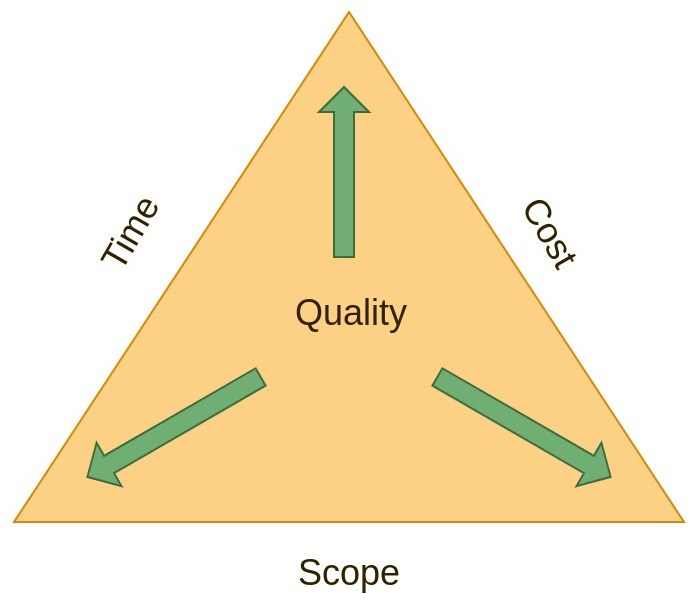
\includegraphics[width=200]{images/quality-triangle.jpg}
    \caption{Representação do triângulo da gestão de um projeto}
\end{figure}

\Par A partir da Figura 1, é possível observar as escolhas que um gestor de projeto tem em relação ao tempo que pretende gastar (\textbf{\textit{Time}}), ao custo total para terminar o projeto (\textbf{\textit{Cost}}) e às funcionalidade que este tem de ter implementadas para ser considerado como terminado (\textbf{\textit{Scope}}). A qualidade do código, que neste contexto estamos a associar ao conceito de \textit{Clean Code}, 
é uma relação direta destas 3 restrições.

\Par No caso de um projeto com tempo limitado, este é o lado do triângulo que será fixo. Se pretendermos manter todas as funcionalidades, teremos de ter em consideração o custo para, por exemplo, contratar mais desenvolvedores de modo a cumprir os prazos estabelecidos no entanto, para isto acontecer, este lado teria de ser flexível, ou seja, o custo tem de suportar aumentos ou diminuições, de modo a manter a uniformidade no triângulo e assegurar o desenvolvimento do projeto.

\Par É usual dizer-se que dentro destas 3 restrições, apenas é possível escolher 2. Logo, pegando no exemplo anterior, muito provavelmente a empresa não estaria interessada em aumentar os custos do projeto, deixando duas opções, ou diminui-se consideravelmente a qualidade do código, ou diminui-se as funcionalidades requeridas, algo que, devido à restrição do tempo, pode também não ser suficiente para assegurar a qualidade. Assim sendo, tendo em conta que muitos dos clientes de uma empresa de desenvolvimento de software apenas querem que um problema esteja resolvido, não estando interessados na qualidade do código, esta acaba por cair para segundo plano. 

\subsection{Conclusão}

\Par Concluindo, \textit{Clean Code} é um conceito extremamente importante para reduzir os custos e tempo despendido na manutenção de um sistema a longo prazo mas, devido às prioridades do mundo empresarial face a um projeto, muitas das vezes estes princípios acabam por cair no esquecimento. Ainda assim, boas práticas como estas são fundamentais na aprendizagem de um desenvolvedor de software, garantido uma maior fiabilidade e robustez nos seus projetos futuros.
 
\clearpage

\section{Referências}

\bibliographystyle{plain}

\bibliography{biblist}

\vspace{5mm} %5mm vertical space

[1] \url{https://gist.github.com/wojteklu/73c6914cc446146b8b533c0988cf8d29}

[2] \url{https://garywoodfine.com/what-is-clean-code/}

[3] \url{https://www.infoq.com/br/articles/clean-code-book-review/}

[4] \url{http://ceur-ws.org/Vol-2066/isee2018paper06.pdf}

[5] \url{https://simpleprogrammer.com/clean-code-principles-better-programmer/}

[6] \url{https://x-team.com/blog/principles-clean-code/}

[7] \url{https://codingsans.com/blog/clean-code}

[8] \url{https://www.hostgator.com.br/blog/clean-code-o-que-e/}

[9] \url{https://www.butterfly.com.au/blog/website-development/clean-high-quality-code-a-guide-on-how-to-become-a-better-programmer}

[11] \url{https://en.wikipedia.org/wiki/Project_management_triangle}

[10] Martin, R. (2009). Clean code : a handbook of agile software craftsmanship. Upper Saddle River, NJ: Prentice Hall.



\end{document}

